\textbf{مورد استفاده:}
داشبورد کاربر
\\
\textbf{شرح مختصر :UC}
در این قسمت دو داشبورد فریلنسر و کارفرما را در اختیار کاربر قرار می‌دهد.
\\
\textbf{پيش شرط:}
ورود به سایت.
\\
\textbf{سناريو اصلی:}
\begin{enumerate}
\item
شروع
\item
کاربر با انتخاب هر کدام از داشبوردها به عنوان کارفرما یا فریلنسر به سیستم معرفی می‌شود.
\item
پایان
\end{enumerate}

\noindent
\textbf{پس شرط:}
ندارد .
\\
\textbf{سناريوهای فرعی:}
ندارد.
\\
\textbf{پس شرط:}
ندارد .
داشبورد-کاربر

\begin{figure}[H]
	\centering
	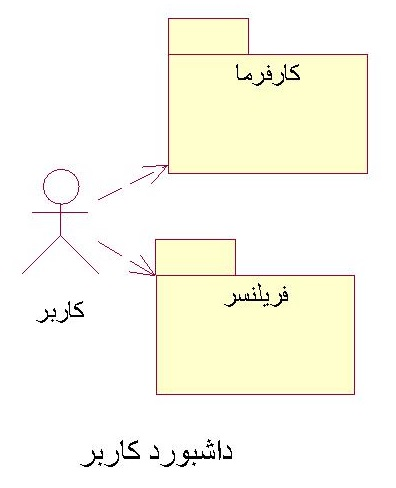
\includegraphics[width=0.4\textwidth]{Diagram/1.UseCase/داشبورد-کاربر.jpg}
	\caption{دیاگرام UC داشبورد کاربر‌}
	\label{fig:uc:داشبورد-کاربر}
\end{figure}
\begin{figure}[H]
%\includegraphics[width=0.7\textwidth]{Diagram/4.Collaboration/-.jpg}
\centering
\caption{دیاگرام همکار داشبورد کاربر}
\label{fig:c:داشبورد-کاربر}
\end{figure}
\begin{figure}[H]
	%\includegraphics[width=0.9\textwidth]{Diagram/2.Activity/-.jpg}
	\centering
	\caption{دیاگرام فعالیت ‌داشبورد کاربر}
	\label{fig:a:داشبورد-کاربر}
\end{figure}
\begin{figure}[H]
	%\includegraphics[width=1\textwidth]{Diagram/3.Sequence/-.jpg}
	\caption{دیاگرام توالی ‌داشبورد کاربر}
	\centering
	\label{fig:s:داشبورد-کاربر}
\end{figure}
